\documentclass[a4paper, 12pt]{article}
\usepackage[utf8x]{inputenc}
\usepackage{cmap}
\usepackage[english, russian]{babel}
\usepackage{indentfirst}
\usepackage[left=20mm, top=20mm, right=20mm, bottom=20mm]{geometry}
\usepackage{tikz}
\usepackage{float}
\usepackage{amsmath, amsfonts, amssymb}
\usepackage{graphicx}
\usepackage{fancybox, fancyhdr}
\usepackage{hyperref}
\usepackage{listings}
\usepackage{caption}
\usepackage{subcaption}
\usepackage{xcolor}
\usepackage{paralist}
\pagestyle{fancy}
\fancyhf{}
\fancyhead[L]{Лабораторная работа №2}
\fancyhead[R]{Моделирование динамических систем}
\fancyfoot[C]{\thepage}
\graphicspath{{images/}}
\usetikzlibrary{patterns}
\definecolor{LightGray}{gray}{0.95}
\definecolor{LightGray2}{gray}{0.7}
\lstdefinestyle{code}{
    language=Python, % replace with needed language
    basicstyle=\footnotesize\ttfamily,
    numbers=left,
    numberstyle=\scriptsize\color{gray},
    stepnumber=1,
    numbersep=5pt,
    backgroundcolor=\color{LightGray},
    showspaces=false,
    showstringspaces=false,
    showtabs=false,
    tabsize=4,
    captionpos=b,
    breaklines=true,
    breakatwhitespace=false,
    frame=single,
    rulecolor=\color{LightGray2},
    linewidth=\linewidth,
    keywordstyle=\color{blue}\bfseries,
    commentstyle=\color{green!40!black},
    stringstyle=\color{purple},
    escapeinside={\%*}{*)},
    inputencoding=utf8x,
    xleftmargin=0pt,
    framexleftmargin=0pt,
    framexrightmargin=0pt
}
\lstset{style=code}
\hypersetup{
    colorlinks=true,
    linkcolor=blue,
    filecolor=magenta,
    urlcolor=cyan,
    pdftitle={contents setup},
    pdfpagemode=FullScreen,
}
\setlength{\parskip}{1.5mm}
\setlength{\headheight}{15pt}
\setlength{\footskip}{15pt}
\allowdisplaybreaks
\DeclareMathOperator{\sinc}{sinc}

\begin{document}
    \begin{titlepage}

        \begin{center}
        
\includegraphics[width=0.3\textwidth]{itmo.png}
        \vfill
        
        Федеральное государственное автономное образовательное учреждение высшего образования
        «Национальный Исследовательский Университет ИТМО»\\
            
        \vfill
        {\large\bf ЛАБОРАТОРНАЯ РАБОТА №2}\\
        {\large\bf ПРЕДМЕТ «МОДЕЛИРОВАНИЕ ДИНАМИЧЕСКИХ СИСТЕМ»}\\
        {\large\bf ТЕМА «НЕЛИНЕЙНЫЕ СИСТЕМЫ УПРАВЛЕНИЯ»}\\
        Вариант 4
        \vfill

        \begin{flushright}
            \begin{minipage}{.45\textwidth}
            {
                \hbox{Преподаватель:}
                \hbox{Семенов Д. М.}
                \hbox{}
                \hbox{Выполнили:}
                \hbox{Румянцев А. А., 368731}
                \hbox{Дьячихин Д. Н., 339080}
                \hbox{Овчинников П. А., 368606}
                \hbox{}
                \hbox{Факультет: СУиР}
            }
            \end{minipage}
        \end{flushright}
        
        \vfill
                
        Санкт-Петербург\\
        2024
        \end{center}
    \end{titlepage}
    
    \tableofcontents

    \newpage
    \section{Задание 1}
    \subsection{Условие}
    Дана нелинейная система
    $$
    \begin{cases}
        \dot{x}=-x-3y,\\
        \dot{y}=-x-4y-\text{sat}\,2y,
    \end{cases}
    \text{ где }
    \text{sat}\,2y=
    \begin{cases}
        2y, & |y|<1\\
        2\,\text{sign}\,y, & |y|\geq1;
    \end{cases}
    $$
    \begin{compactitem}
    \item найти ее положения равновесия;
    \item линеаризовать систему около одного из положений равновесия,
    исследовать полученную систему на устойчивость;
    \item доказать устойчивость исходной системы с помощью метода
    функций Ляпунова;
    \item построить графики исходной и линеаризованной систем.
    \end{compactitem}


    \subsection{Выполнение}
    Рассмотрим $|y|<1$. Система примет вид
    $$
    \begin{cases}
        \dot{x}=-x-3y\\
        \dot{y}=-x-4y-2y
    \end{cases}
    \Rightarrow
    \begin{cases}
        \dot{x}=-x-3y\\
        \dot{y}=-x-6y
    \end{cases}
    $$
    Найдем положения равновесия: $\dot{x}=0,\,\dot{y}=0$
    $$
    \begin{cases}
        -x-3y=0\\
        -x-6y=0
    \end{cases}
    \Rightarrow
    \begin{cases}
        x=-3y\\
        3y-6y=0
    \end{cases}
    \Rightarrow
    \begin{cases}
        x=0\\
        y=0
    \end{cases}
    \Rightarrow
    x^*=\begin{bmatrix}
        0\\
        0
    \end{bmatrix}
    $$


    Линеаризуем исследуемую систему в окрестности положения равновесия (0, 0):
    $$
    J(x)=
    \begin{bmatrix}
        f^{\prime}_{1x} & f^{\prime}_{1y}\\
        f^{\prime}_{2x} & f^{\prime}_{2y}
    \end{bmatrix}=
    \begin{bmatrix}
        -1 & -3\\
        -1 & -6
    \end{bmatrix},\ \
    \dot{x}=J|_{x=x^*}=Ax=
    \begin{bmatrix}
        -1 & -3\\
        -1 & -6
    \end{bmatrix}x
    $$
    Определим тип положения равновесия (0, 0). Для этого найдем собственные
    числа матрицы $A$ и исследуем их:
    $$
    \det{\{\lambda I-A\}}=
    \begin{vmatrix}
        \lambda+1 & 3\\
        1 & \lambda+6
    \end{vmatrix}=
    \left(\lambda+1\right)\left(\lambda+6\right)-3=0\Rightarrow
    \lambda_{1,2}=-3.5\pm\sqrt{9.25}
    $$
    $$
    \lambda_1=-3.5+\sqrt{9.25}\approx-0.46<0,\ \ \lambda_2=-3.5-\sqrt{9.25}\approx-6.54<0
    $$
    Так как собственные числа действительные, отрицательные и, не равны, то положение равновесия -- устойчивый узел.


    Введем функцию Ляпунова $V(x)=x^2+y^2$ для исследования глобальной устойчивости
    системы. Покажем, что при данной функции Ляпунова выполняется теорема об асимптотической
    устойчивости:
    $$
    \dot{V}(x)=2x\dot{x}+2y\dot{y}=2x\left(-x-3y\right)+2y\left(-x-6y\right)=-2x^2-8xy-12y^2,
    $$
    $$
    -2x^2-8xy-12y^2=-2\left(x^2+4xy+6y^2\right)=-2\left(x^2+4xy+4y^2+2y^2\right)=-2\left(\left(x+2y\right)^2+2y^2\right)
    $$
    Из последнего имеем (при условии $|y|<1$)
    $$
    \begin{cases}
        \left(x+2y\right)^2>0,\ \forall x\\
        2y^2>0,\ \forall y\\
        -2\cdot\left(\text{sum of positives}\right)
    \end{cases}\Rightarrow
    \dot{V}(x)<0,\ \forall x\in\mathbb{R}^2\,\backslash\,\{0\}
    $$
    Следовательно, для введенной функции $V(x)$ и исследуемой системы выполняются
    условия теоремы об асимптотической устойчивости, а значит, нулевое решение системы
    глобально асимптотически устойчиво.


    Рассмотрим $|y|\geq1$. Получим систему
    $$
    \begin{cases}
        \dot{x}=-x-3y\\
        \dot{y}=-x-4y-2\,\text{sign}\,y
    \end{cases}
    $$
    Здесь будет еще два случая: $y\leq-1$ и $y\geq1$. Системы будут иметь вид
    $$
    y\leq-1:
    \begin{cases}
        \dot{x}=-x-3y,\\
        \dot{y}=-x-4y+2,
    \end{cases}\ \ 
    y\geq1:
    \begin{cases}
        \dot{x}=-x-3y\\
        \dot{y}=-x-4y-2
    \end{cases}
    $$
    Аналогично найдем положения равновесия:
    $$
    y\leq-1:
    \begin{cases}
        -x-3y=0,\\
        -x-4y+2=0,
    \end{cases}\ \ 
    y\geq1:
    \begin{cases}
        -x-3y=0\\
        -x-4y-2=0
    \end{cases}
    $$
    $$
    y\leq-1:
    \begin{cases}
        x=-3y,\\
        3y-4y+2=0,
    \end{cases}\ \ 
    y\geq1:
    \begin{cases}
        x=-3y\\
        3y-4y-2=0
    \end{cases}
    $$
    $$
    y\leq-1:
    \begin{cases}
        x=-6,\\
        y=2>0\text{ (не уд. усл.)},
    \end{cases}\ \ 
    y\geq1:
    \begin{cases}
        x=6\\
        y=-2<0\text{ (не уд. усл.)}
    \end{cases}
    $$
    В обоих случаях положения равновесия имеют координату $y$, не удовлетворяющую соответствующим условиям, заданным на $y$.
    Мы не можем линеаризовать системы.
    
    Если применить метод функции Ляпунова, то константа $\pm2$ не позволит
    знакоопределить $\dot{V}(x)$, так как получится неквадратная составляющая $ay$, где $a$ -- некоторый коэффициент.
    Для знакоопределения функции Ляпунова необходимы составляющие вида $ax^2,\,by^2,\,cxy$, где $a,\,b,\,c$ -- константы.
    Таким образом, устойчивость исходной системы в этих областях остаётся неопределённой.


    Графики исходной и линеаризованной систем изображены на рис \ref{fig:task1}. Программа для построения графиков представлена на листинге \ref{task1code}.
    \begin{figure}[H]
        \centering
        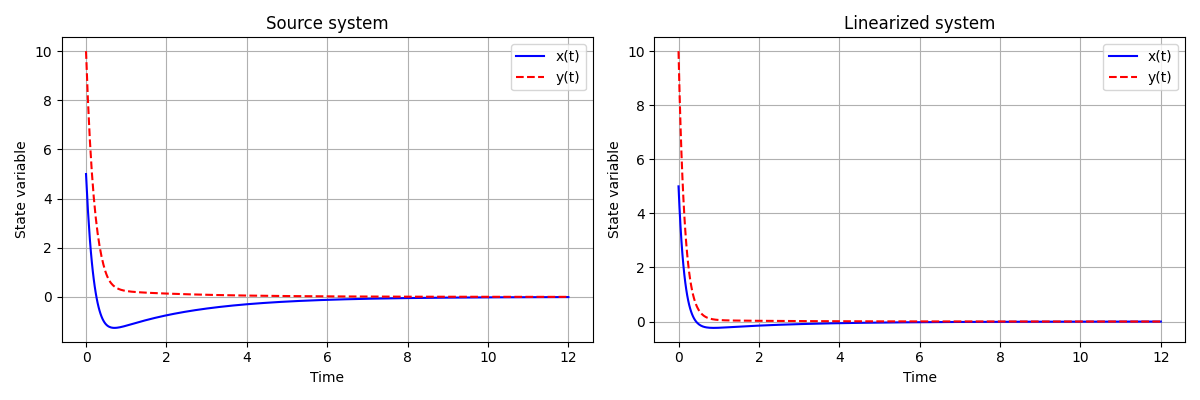
\includegraphics[scale=0.55]{task1.png}
        \captionsetup{skip=0pt}
        \caption{Динамика исследуемой динамической системы}
        \label{fig:task1}
    \end{figure}


    \section{Задание 2}
    \subsection{Условие}
    Дана нелинейная система
    $$
    \dot{x}=Ax+b\xi,\ \ \sigma=c^Tx,\ \ \xi=\varphi(\sigma,t),
    $$
    где
    $$
    A=
    \begin{bmatrix}
        -1 & 2\\
        -2 & -2
    \end{bmatrix},\ \
    b=
    \begin{bmatrix}
        1\\
        0
    \end{bmatrix},\ \
    c=
    \begin{bmatrix}
        1\\
        0
    \end{bmatrix},\ \
    \xi=
    \dfrac{\sigma}{|\sigma|+2};
    $$
    С помощью кругового критерия доказать экспоненциальную устойчивость системы.


    \subsection{Выполнение}
    Проверим выполнение всех пунктов критерия.
    \begin{compactitem}
        \item Выполнение <<секторного условия>>:
        $$\mu_1\leq\varphi(\sigma)/\sigma\leq\mu_2,\ \ \sigma\neq0,\ \ \forall t\in(0,\infty)$$
        В нашем случае
        $$\varphi(\sigma)/\sigma=\dfrac{\sigma}{|\sigma|+2}\div \sigma=\dfrac{1}{|\sigma|+2},$$
        $$\mu_1\leq\dfrac{1}{|\sigma|+2}\leq\mu_2$$
        Рассмотрим пределы, чтобы найти $\mu_1,\,\mu_2$:
        $$\lim\limits_{\sigma\to\infty}\dfrac{1}{|\sigma|+2}=\left\{\dfrac{1}{\infty}\right\}=\mu_1=0,$$
        $$\lim\limits_{\sigma\to0}\dfrac{1}{|\sigma|+2}=\left\{\dfrac{1}{0+2}\right\}=\mu_2=\dfrac{1}{2}$$
        Получаем $\mu_1=0,\,\mu_2=0.5$. График $\varphi(\sigma)$ представлен на рис. \ref{fig:task2}.
        Программа для построения графика представлена на листинге \ref{task2code}.
        \begin{figure}[H]
            \centering
            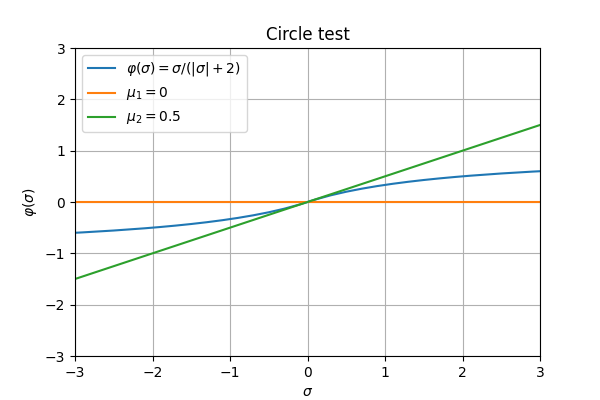
\includegraphics[scale=0.55]{task2.png}
            \captionsetup{skip=0pt}
            \caption{Круговой критерий: выполнение секторного условия для системы}
            \label{fig:task2}
        \end{figure}
        Из рис. \ref{fig:task2} следует, что <<секторное условие>> выполнено.
        \item Наличие у матрицы $A$ чисто мнимых собственных значений:
        $$
        \det{\{\lambda I-A\}}=
        \begin{vmatrix}
            \lambda+1 & -2\\
            2 & \lambda+2
        \end{vmatrix}=
        (\lambda+1)(\lambda+2)+4=0,
        $$
        $$
        (\lambda+1)(\lambda+2)+4=\lambda^2+3\lambda+6=0\Rightarrow
        \lambda_{1,2}=-1.5\pm i\sqrt{3.75}
        $$
        Матрица $A$ не имеет чисто мнимых собственных значений $\Rightarrow$ условие выполнено.
        \item Асимптотическая устойчивость системы при $\xi=\mu_0\sigma$. Поскольку значение
        $\mu_0$ выбирается из интервала $\left[\mu_1,\mu_2\right]$, то можно выбрать
        $\mu_0=\mu_1=0$. Тогда исследуемая система будет иметь вид $\dot{x}=Ax$.
        Поскольку собственные числа матрицы $A$ уже известны $\Re\left\{\lambda_{1,2}\right\}<0$,
        то матрица $A$ устойчива $\Rightarrow$ линейная система асимптотически устойчива, а значит,
        условие выполнено.
        \item Выполнение <<частотного условия>>. Для начала найдем передаточную функцию $W(\lambda)$.
        По определению имеем $$W(\lambda)=c^T(A-\lambda I)^{-1}b$$ В нашем случае
        $$(A-\lambda I)^{-1}=
        \begin{bmatrix}
            -1-\lambda & 2\\
            -2 & -2-\lambda
        \end{bmatrix}^{-1}=
        \dfrac{1}{\lambda^2+3\lambda+6}
        \begin{bmatrix}
            -\lambda-2 & -2\\
            2 & -\lambda-1
        \end{bmatrix},$$
        $$
        c^T(A-\lambda I)^{-1}=
        \dfrac{1}{\lambda^2+3\lambda+6}
        \begin{bmatrix}
            1 & 0
        \end{bmatrix}
        \begin{bmatrix}
            -\lambda-2 & -2\\
            2 & -\lambda-1
        \end{bmatrix}=
        \dfrac{1}{\lambda^2+3\lambda+6}
        \begin{bmatrix}
            -\lambda-2 & -2
        \end{bmatrix},
        $$
        $$
        c^T(A-\lambda I)^{-1}b=
        \dfrac{1}{\lambda^2+3\lambda+6}
        \begin{bmatrix}
            -\lambda-2 & -2
        \end{bmatrix}
        \begin{bmatrix}
            1\\
            0
        \end{bmatrix}=
        \dfrac{-\lambda-2}{\lambda^2+3\lambda+6}=W(\lambda)
        $$
        Таким образом, $$W(\lambda)=\dfrac{-\lambda-2}{\lambda^2+3\lambda+6}$$
        Зададим $\lambda=i\omega$ и проверим выполнение неравенства
        $$\Re\left\{\left[1+\mu_1W(i\omega)\right]\left[1+\mu_2W(i\omega)\right]^*\right\}>0,\ \ \omega\in(-\infty,+\infty)$$
        Поскольку $\mu_1=0$ и $\mu_2=0.5$, получаем, что должно быть выполнено неравенство
        $$\Re\left\{\left[1+0.5W(i\omega)\right]^*\right\}>0,\ \ \omega\in(-\infty,+\infty)$$
        В нашем случае $$0.5W(i\omega)=\dfrac{-2-i\omega}{2\left(i^2\omega^2+3i\omega+6\right)}=\dfrac{-2-i\omega}{2\left(-\omega^2+3i\omega+6\right)},$$
        $$1+0.5W(i\omega)=1+\dfrac{-2-i\omega}{2\left(-\omega^2+3i\omega+6\right)}=\dfrac{-\omega^2+2.5i\omega+5}{-\omega^2+3i\omega+6},$$
        $$\dfrac{-\omega^2+2.5i\omega+5}{-\omega^2+3i\omega+6}=\dfrac{(-\omega^2+2.5i\omega+5)((6-\omega^2)-3i\omega)}{((6-\omega^2)+3i\omega)((6-\omega^2)-3i\omega)}=
        \dfrac{\omega^4+0.5i\omega^3-3.5\omega^2+30}{(6-\omega^2)^2+9\omega^2},$$
        $$\Re\left\{\dfrac{\omega^4+0.5i\omega^3-3.5\omega^2+30}{(6-\omega^2)^2+9\omega^2}\right\}=\dfrac{\omega^4-3.5\omega^2+30}{(6-\omega^2)^2+9\omega^2}$$
        Знаменатель всегда положителен. Рассмотрим числитель -- выделим в нем квадраты, если возможно
        $$\omega^4-3.5\omega^2+30=\omega^4-3.5\omega^2+1.75^2+(30-1.75^2)=(\omega^2-1.75)^2+26.9375$$
        Теперь получим
        $$\Re\left\{\left[1+0.5W(i\omega)\right]^*\right\}=\dfrac{(\omega^2-1.75)^2+26.9375}{(6-\omega^2)^2+9\omega^2}>0,\ \ \omega\in(-\infty,+\infty)$$
        Числитель и знаменатель полученной дроби положительны $\forall\omega$. Все условия теоремы выполнены,
        следовательно, система экспоненциально устойчива.
    \end{compactitem}


    \section{Задание 3}
    \subsection{Условие}
    Дана нелинейная система
    $$
    \dot{x}=Ax+b\xi,\ \ \sigma=c^Tx,\ \ \xi=\varphi(\sigma),
    $$
    где
    $$
    A=
    \begin{bmatrix}
        -1 & -2\\
        4 & -2
    \end{bmatrix},\ \
    b=
    \begin{bmatrix}
        1\\
        0
    \end{bmatrix},\ \
    c=
    \begin{bmatrix}
        0\\
        1
    \end{bmatrix},\ \
    \xi=
    \dfrac{\sigma}{|\sigma|+3};
    $$
    С помощью критерия Попова доказать асимптотическую устойчивость системы.


    \subsection{Выполнение}
    Проверим выполнение всех пунктов критерия.
    \begin{compactitem}
        \item Выполнение <<секторного условия>>: $$0\leq\varphi(\sigma)/\sigma\leq\mu_0\leq+\infty,\ \ \sigma\neq0,\ \ \forall t\in(0,\infty)$$
        В нашем случае
        $$\varphi(\sigma)/\sigma=\dfrac{\sigma}{|\sigma|+3}\div \sigma=\dfrac{1}{|\sigma|+3}$$
        Чтобы найти $\mu_0$, рассмотрим предел в нуле справа (производной в точке $\sigma=0$ не существует)
        $$\lim\limits_{\sigma\to+0}\dfrac{1}{|\sigma|+3}=\left\{\dfrac{1}{|+0|+3}\right\}=\mu_0=\dfrac{1}{3}$$
        Получаем $\mu_0=1/3$. График $\varphi(\sigma)$ представлен на рис. \ref{fig:task3}.
        Программа для построения графика представлена на листинге \ref{task3code}.
        \begin{figure}[H]
            \centering
            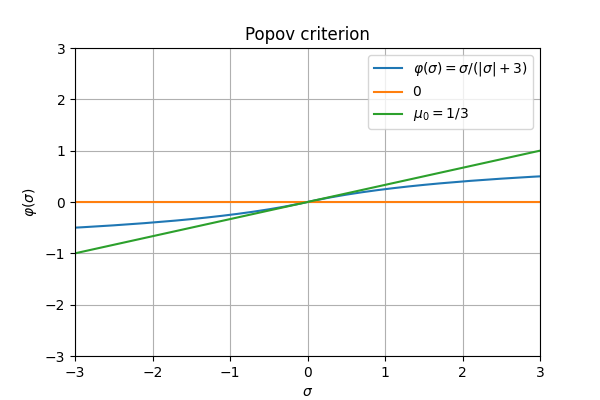
\includegraphics[scale=0.55]{task3.png}
            \captionsetup{skip=0pt}
            \caption{Критерий Попова: выполнение секторного условия для системы}
            \label{fig:task3}
        \end{figure}
        \item Устойчивость матрицы $A$:
        $$\det{\{\lambda I-A\}}=
        \begin{vmatrix}
            \lambda+1 & 2\\
            -4 & \lambda+2
        \end{vmatrix}=
        (\lambda+1)(\lambda+2)+8=0,$$
        $$(\lambda+1)(\lambda+2)+8=\lambda^2+3\lambda+10=0\Rightarrow\lambda_{1,2}=-1.5\pm i\sqrt{7.75}$$
        Так как $\Re\left\{\lambda_{1,2}\right\}<0,\,\lambda_1\neq\lambda_2$, то матрица $A$ устойчива.
        \item Выполнение <<частотного условия>>. Для начала найдем передаточную функцию $W(\lambda)$
        аналогично заданию 2: $$W(\lambda)=c^T(A-\lambda I)^{-1}b,$$
        $$(A-\lambda I)^{-1}=
        \begin{bmatrix}
            -1-\lambda & -2\\
            4 & -2-\lambda
        \end{bmatrix}^{-1}=
        \dfrac{1}{\lambda^2+3\lambda+10}
        \begin{bmatrix}
            -\lambda-2 & 2\\
            -4 & -\lambda-1
        \end{bmatrix},$$
        $$
        c^T(A-\lambda I)^{-1}=
        \dfrac{1}{\lambda^2+3\lambda+10}
        \begin{bmatrix}
            0 & 1
        \end{bmatrix}
        \begin{bmatrix}
            -\lambda-2 & 2\\
            -4 & -\lambda-1
        \end{bmatrix}=
        \dfrac{1}{\lambda^2+3\lambda+10}
        \begin{bmatrix}
            -4 & -\lambda-1
        \end{bmatrix},
        $$
        $$
        c^T(A-\lambda I)^{-1}b=
        \dfrac{1}{\lambda^2+3\lambda+10}
        \begin{bmatrix}
            -4 & -\lambda-1
        \end{bmatrix}
        \begin{bmatrix}
            1\\
            0
        \end{bmatrix}=
        \dfrac{-4}{\lambda^2+3\lambda+10}=W(\lambda)
        $$
        Таким образом, $$W(\lambda)=\dfrac{-4}{\lambda^2+3\lambda+10}$$
        Возьмем $\lambda=i\omega$ и проверим выполнение неравенства
        $$\mu_0^{-1}+\Re\left\{(1+i\omega\nu)W(i\omega)\right\}>0,\ \ \forall\omega\in[0,+\infty)$$
        Учитывая, что $\mu_0^{-1}|_{\mu_0=1/3}=3$, получаем, что должно быть выполнено неравенство
        $$3+\Re\left\{(1+i\omega\nu)W(i\omega)\right\}>0,\ \ \forall\omega\in[0,+\infty)$$
        Имеем
        $$W(i\omega)=\dfrac{-4}{-\omega^2+3i\omega+10},\ \ (1+i\omega\nu)W(i\omega)=\dfrac{-4-4i\omega\nu}{-\omega^2+3i\omega+10},$$
        $$\dfrac{-4-4i\omega\nu}{-\omega^2+3i\omega+10}=\dfrac{(-4-4i\omega\nu)((10-\omega^2)-3i\omega)}{((10-\omega^2)+3i\omega)((10-\omega^2)-3i\omega)},$$
        $$\dfrac{(-4-4i\omega\nu)((10-\omega^2)-3i\omega)}{((10-\omega^2)+3i\omega)((10-\omega^2)-3i\omega)}=\dfrac{-40+4\omega^2-12\omega^2\nu+(12\omega-40\omega\nu+4\omega^3\nu)i}{(10-\omega^2)^2+9\omega^2},$$
        $$\Re\left\{\dfrac{-40+4\omega^2-12\omega^2\nu+(12\omega-40\omega\nu+4\omega^3\nu)i}{(10-\omega^2)^2+9\omega^2}\right\}=\dfrac{4\omega^2-12\omega^2\nu-40}{(10-\omega^2)^2+9\omega^2},$$
        $$3+\Re\left\{(1+i\omega\nu)W(i\omega)\right\}=3+\dfrac{4\omega^2-12\omega^2\nu-40}{(10-\omega^2)^2+9\omega^2}=\dfrac{3\omega^4+\omega^2(-29-12\nu)+260}{(10-\omega^2)^2+9\omega^2}$$
        Знаменталь всегда больше нуля. Рассмотрим числитель:
        $$
        \begin{matrix}
            3\omega^4\geq0,\ \forall\omega\geq0,\\
            \omega^2\geq0,\ \forall\omega\geq0,\\
            260>0,\\
            -29-12\nu\,?\,0
        \end{matrix}
        $$
        По условию теоремы, при некоторых $\nu$ должно выполняться <<частотное условие>>.
        В таком случае необходимо, чтобы $$-29-12\nu\geq0\Rightarrow12\nu\leq-29\Rightarrow\nu\leq-\dfrac{29}{12}$$
        Таким образом,
        $$\dfrac{3\omega^4+\omega^2(-29-12\nu)+260}{(10-\omega^2)^2+9\omega^2}>0$$
        При $\nu\leq-29/12$ числитель и знаменатель
        полученной дроби положительны при $\forall\omega$.
        Все условия теоремы выполнены, следовательно, система
        асимптотически устойчива.
    \end{compactitem}


    \section{Вывод}
    В ходе выполнения лабораторной работы были
    решены задачи анализа и исследования нелинейных систем.


    Мы доказали устойчивость исходной системы задания 1 методами
    линеаризации вблизи одного из положений равновесия и функцией
    Ляпунова. Мы проверили себя, построив графики исходной и линеаризованной систем.


    Экспоненциальная устойчивость нелинейной системы задания 2 была
    подтверждена с использованием кругового критерия -- мы проверили
    соблюдение всех условий, в частности исследовали <<частотное условие>>,
    для которого искали передаточную функцию. Мы проверили себя, построив
    график нелинейной системы вместе с полученными с помощью
    предельного исследования значениями ограничений.


    Аналогичным способом асимптотическая устойчивость
    системы задания 3 была доказана с помощью критерия Попова.
    

    \section{Приложения}
    Программа для задания 1.
    \begin{lstlisting}[label=task1code, caption={Программа для построения исходной и линеаризованной систем}]
    import numpy as np
    from scipy.integrate import solve_ivp
    import matplotlib.pyplot as plt

    def sat(par):
        if np.abs(par) < 1:
            return par
        return np.sign(par)

    def nonlinear_system(t, y):
        x1, x2 = y
        dx1_dt = -x1 - 3 * x2
        dx2_dt = -x1 - 4 * x2 - 2 * sat(x2)
        return [dx1_dt, dx2_dt]

    def linearized_system(t, y):
        x1, x2 = y
        dx1_dt = -x1 - 3 * x2
        dx2_dt = -x1 - 6 * x2
        return [dx1_dt, dx2_dt]

    x0 = [5.0, 10.0]
    t_span = (0, 12)
    t_eval = np.linspace(t_span[0], t_span[1], 500)
    src_sol = solve_ivp(nonlinear_system, t_span, x0,
                        method='RK45', t_eval=t_eval)
    lin_sol = solve_ivp(linearized_system, t_span, x0,
                        method='RK45', t_eval=t_eval)
    fig, axes = plt.subplots(1, 2, figsize=(12, 4))
    axes[0].plot(src_sol.t, src_sol.y[0], label='x(t)', color='b')
    axes[0].plot(src_sol.t, src_sol.y[1], label='y(t)', color='r',
                linestyle='--')
    axes[0].set_title('Source system')
    axes[0].set_xlabel('Time')
    axes[0].set_ylabel('State variable')
    axes[0].grid(True)
    axes[0].legend()
    axes[1].plot(lin_sol.t, lin_sol.y[0], label='x(t)', color='b')
    axes[1].plot(lin_sol.t, lin_sol.y[1], label='y(t)', color='r',
                linestyle='--')
    axes[1].set_title('Linearized system')
    axes[1].set_xlabel('Time')
    axes[1].set_ylabel('State variable')
    axes[1].grid(True)
    axes[1].legend()
    plt.tight_layout()
    plt.show()
    \end{lstlisting}


    Программа для задания 2.
    \begin{lstlisting}[label=task2code, caption={Программа для построения графика $\varphi(\sigma)$}]
    import matplotlib.pyplot as plt
    import numpy as np

    sigma = np.linspace(-100, 100, 1000)
    mu1 = 0
    mu2 = 1 / 2
    plt.plot(sigma, sigma / (np.abs(sigma) + 2),
            label=r'$\varphi(\sigma)=\sigma/(|\sigma|+2)$')
    plt.plot(sigma, mu1 * sigma, label=r'$\mu_1=0$')
    plt.plot(sigma, mu2 * sigma, label=r'$\mu_2=0.5$')
    plt.title('Circle test')
    plt.xlabel(r'$\sigma$')
    plt.ylabel(r'$\varphi(\sigma)$')
    plt.xlim(-3, 3)
    plt.ylim(-3, 3)
    plt.grid()
    plt.legend()
    plt.gcf().set_size_inches(6, 4)
    plt.show()
    \end{lstlisting}


    Программа для задания 3.
    \begin{lstlisting}[label=task3code, caption={Программа для построения графика $\varphi(\sigma)$}]
    import matplotlib.pyplot as plt
    import numpy as np

    sigma = np.linspace(-100, 100, 1000)
    mu1 = 0
    mu2 = 1 / 3
    plt.plot(sigma, sigma / (np.abs(sigma) + 3),
            label=r'$\varphi(\sigma)=\sigma/(|\sigma|+3)$')
    plt.plot(sigma, mu1 * sigma, label='0')
    plt.plot(sigma, mu2 * sigma, label=r'$\mu_0=1/3$')
    plt.title('Popov criterion')
    plt.xlabel(r'$\sigma$')
    plt.ylabel(r'$\varphi(\sigma)$')
    plt.xlim(-3, 3)
    plt.ylim(-3, 3)
    plt.grid()
    plt.legend()
    plt.gcf().set_size_inches(6, 4)
    plt.show()
    \end{lstlisting}
\end{document}